\begin{figure}[t]
\centering
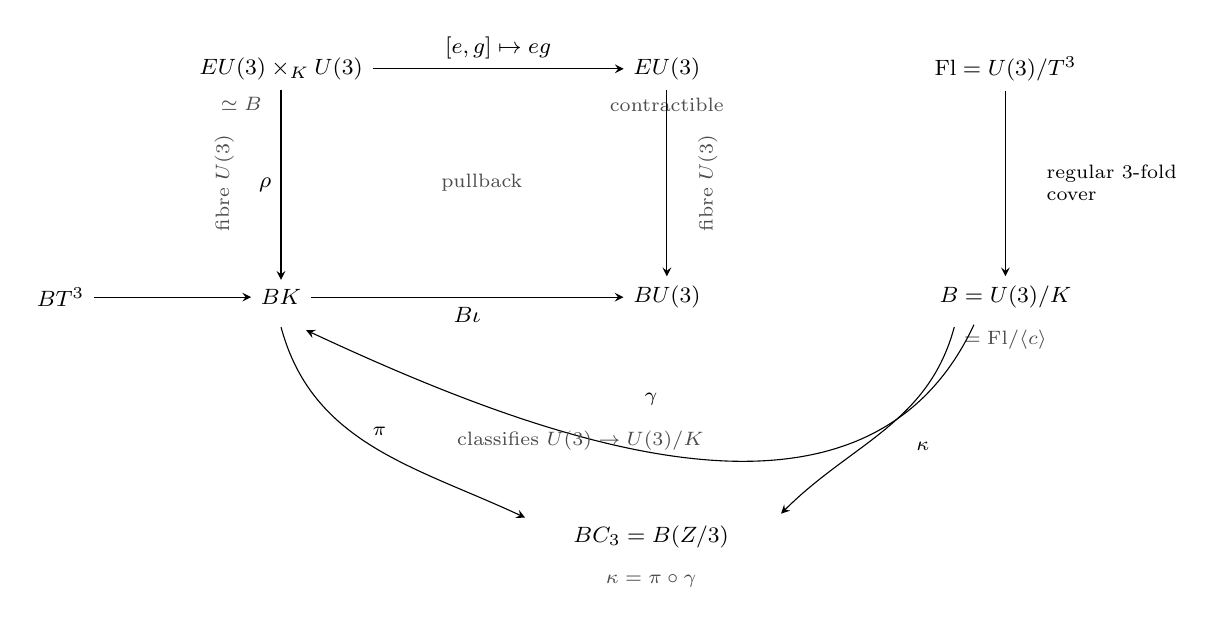
\begin{tikzpicture}[>=stealth, every node/.style={font=\footnotesize}]
  % Borel pullback square (Step 1)
  \node (E) at (0.3,3.3) {$EU(3)\times_K U(3)$};
  \node[anchor=east, font=\scriptsize, text=gray!60!black] at (0.18,2.86) {$\simeq B$};
  \node (F) at (5.2,3.3) {$EU(3)$};
  \node[font=\scriptsize, text=gray!60!black] at (5.2,2.84) {contractible};
  \node (G) at (0.3,0.4) {$BK$};
  \node (H) at (5.2,0.4) {$BU(3)$};
  \draw[->] (E) -- (F) node[midway, above] {$[e,g]\mapsto eg$};
  \draw[->] (E) -- (G) node[midway, left] {$\rho$};
  \draw[->] (F) -- (H);
  \draw[->] (G) -- (H) node[midway, below] {$B\iota$};
  \node[font=\scriptsize, rotate=90, text=gray!60!black] at (-0.42,1.85) {fibre $U(3)$};
  \node[font=\scriptsize, rotate=90, text=gray!60!black] at (5.72,1.85) {fibre $U(3)$};
  \node[font=\scriptsize, text=gray!60!black] at (2.85,1.85) {pullback};
  % quotient tower and classifying maps (Steps 0 and 6)
  \node (FL) at (9.5,3.3) {$\mathrm{Fl}=U(3)/T^3$};
  \node (BN) at (9.5,0.4) {$B=U(3)/K$};
  \node[font=\scriptsize, text=gray!60!black] at (9.5,-0.14) {$=\mathrm{Fl}/\langle c\rangle$};
  \draw[->] (FL) -- (BN);
  \node[right, font=\scriptsize, align=left] at (9.9,1.85) {regular $3$-fold\\cover};
  \draw[->] (9.1,0.05) to[out=245,in=335] (0.62,-0.02);
  \node[font=\scriptsize] at (5.0,-0.9) {$\gamma$};
  \node[font=\scriptsize, text=gray!60!black] at (4.1,-1.42) {classifies $U(3)\to U(3)/K$};
  \node (BT) at (-2.5,0.4) {$BT^3$};
  \draw[->] (BT) -- (G);
  \node (BC) at (5.0,-2.65) {$BC_3=B(\mathbb Z/3)$};
  \draw[->] (0.3,0.02) to[out=285,in=155] (3.4,-2.4);
  \node[font=\scriptsize] at (1.55,-1.3) {$\pi$};
  \draw[->] (8.85,0.02) to[out=255,in=45] (6.65,-2.35);
  \node[font=\scriptsize] at (8.45,-1.5) {$\kappa$};
  \node[font=\scriptsize, text=gray!60!black] at (5.0,-3.2) {$\kappa=\pi\circ\gamma$};
\end{tikzpicture}
\caption{The spaces and maps of the proof of Proposition~\ref{prop:cupsquare}. Left: the Borel bundle of Step~1, a fibre bundle with fibre $U(3)$, total space $EU(3)\times_KU(3)$ homotopy equivalent to $B$, and base $BK$; it is the pullback of the universal bundle $U(3)\to EU(3)\to BU(3)$ along $B\iota\colon BK\to BU(3)$, with $[e,g]\mapsto eg$ on top and $BK=EC_3\times_{C_3}BT^3$ as in Step~2. Right: the homogeneous models of Step~0, the flag manifold $\mathrm{Fl}=U(3)/T^3$ and the quotient $B=U(3)/K=\mathrm{Fl}/\langle c\rangle$ under the regular three-fold cover with deck group $\langle c\rangle\cong\mathbb Z/3$, together with the classifying maps of Step~6: $\gamma$ classifies the principal $K$-bundle $U(3)\to U(3)/K$, $\pi$ is the quotient $BK\to BC_3$, and $\kappa=\pi\circ\gamma$ classifies the cover. The arrow $BT^3\to BK$ is the fibre of the fibration of Step~2. Under the identification of the total space with $B$, the projection $\rho$ equals $\gamma$; the deck transformation $c$ acts by right multiplication by the permutation matrix $\sigma$, and $K=T^3\rtimes\langle\sigma\rangle$ (Step~0).}
\label{fig:flag-fibration}
\end{figure}
